\begin{frame}{Future Work}
	\begin{itemize}
		\item Distributed server architecture, different filters for different licenses
		\item Bloom Filter very old, slightly better solutions available
		\item Method based approach instead of indexing complete file
		\item Community driven marking of irrelevant hits
	\end{itemize}
\end{frame}


\begin{frame}{Sorting Tags}
	\centering
	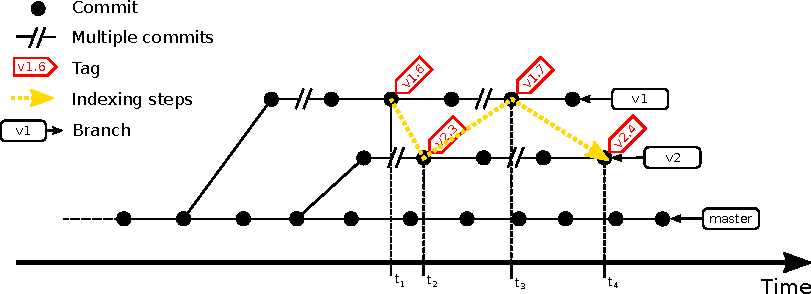
\includegraphics[width=\linewidth]{../written/figures/tag_sort.pdf}
\end{frame}

\begin{frame}
	Code Beispiele 
\end{frame}

\begin{frame}{Definition of infringement}
\begin{itemize}
	\item Study on Uniqueness of Code \cite{2010-gabel-su-source-code-uniqueness}:\\
	\textit{\enquote{general lack of uniqueness in [...] one to seven lines of source code}}
	\item Veritas Operating Corp. vs Microsoft Corp \cite{mertzel2008copying}:
	\textit{54 out of 160.000 lines of code copied}
\end{itemize}

\begin{center}
	\textbf{$\rightarrow$ 8 lines minimum, 54 critical}
\end{center}
Identical code fragments, excerpt whitespace and comments with changed, added or removed statements
\note{
	\begin{itemize}
		\item Kopie $\rightarrow$ Lizenzverletzung?
		\item Zwei Anhaltspunkte
		\item Trotzdem: abhängig inhalt
	\end{itemize}
}
\end{frame}